% Copyright (C)  2014 Richard Bäck.
% Permission is granted to copy, distribute and/or modify this document
% under the terms of the GNU Free Documentation License, Version 1.3 or
% any later version published by the Free Software Foundation; with no
% Invariant Sections, no Front-Cover Texts, and no Back-Cover Texts.  A
% copy of the license is included in the section entitled "GNU Free
% Documentation License".

\documentclass[a4paper,10pt]{report}
\usepackage{amsmath}
\usepackage[utf8]{inputenc}
\usepackage{palatino}
\usepackage{graphicx}
\usepackage{fancyhdr}
\usepackage{eurosym}
\usepackage{hyperref}
\usepackage{multicol}
\usepackage{titlesec}
\usepackage[german]{babel}
\usepackage[margin=1.5cm,vmargin={0pt,1cm}]{geometry}

\DeclareGraphicsExtensions{.pdf}

\setlength{\headheight}{2.5cm}
\setlength{\headsep}{0.5cm}
\setlength{\textheight}{25.2cm}

\pagestyle{fancy}
\lhead{Richard Bäck}
\chead{}
\rhead{\today}
\lfoot{Das Anlagevermögen \& die Anlagenabschreibung}
\cfoot{}
\rfoot{Seite \thepage}
\renewcommand{\headrulewidth}{0.4pt}
\renewcommand{\footrulewidth}{0.4pt}

\newcommand\tkonto[3]{
\begin{tabular}{l|l}
  \multicolumn{2}{c}{#1}\\
  \hline
  #2 & #3
\end{tabular}}

\titleclass{\chapter}{straight}
\titleformat{\chapter}[display]
  {\normalfont\huge\bfseries}{\chaptertitlename\ \thechapter}{20pt}{\Huge}
\titlespacing*{\chapter} {0pt}{50pt}{40pt}

\title{Das Anlagevermögen \& die Anlagenabschreibung}
\author{Richard Bäck}

\begin{document}

\maketitle
\tableofcontents
\pagebreak
\listoffigures
\pagebreak
\listoftables
\pagebreak

\chapter{Ein kurzer Überblick über die Themen}
\begin{figure}[ht]
\centering
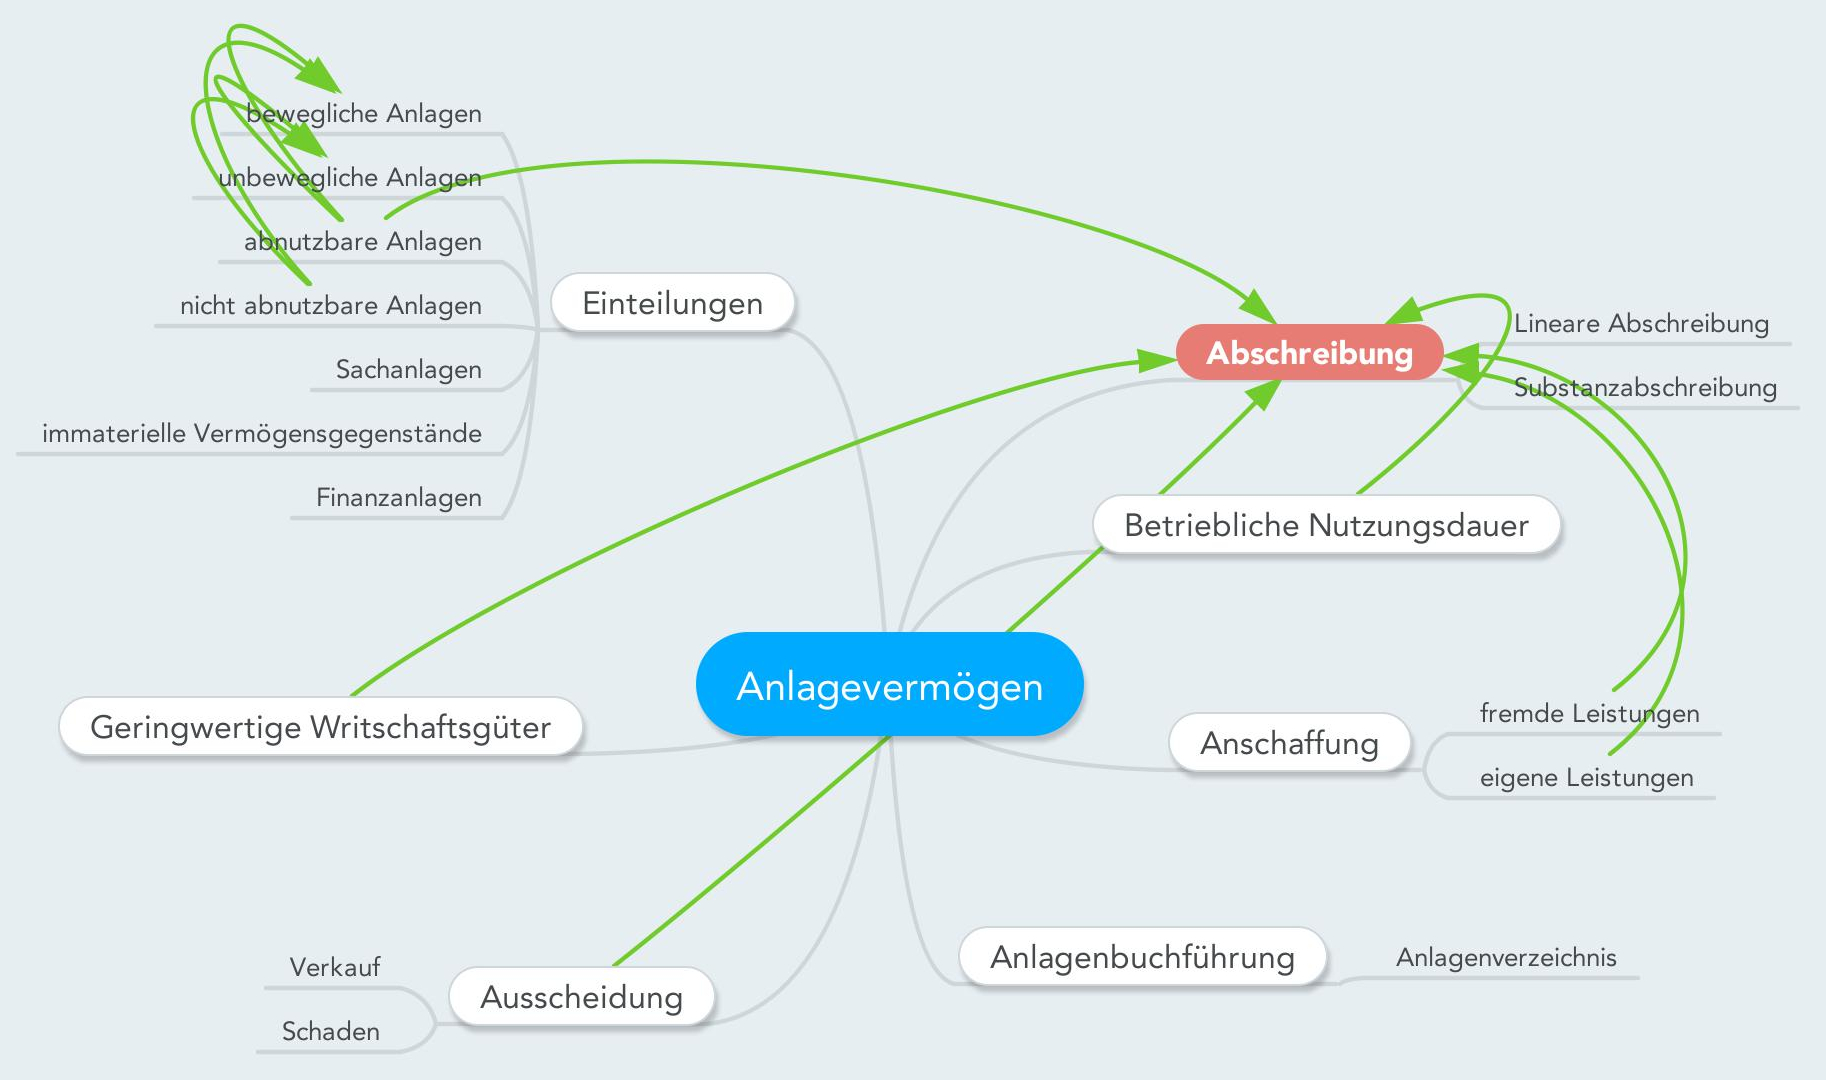
\includegraphics[width=18cm]{Bilder/Ueberblick}
\caption{Überlich über das Thema des Anlagevermögens}
\end{figure}


\chapter{Das Anlagevermögen}
\thispagestyle{fancy}
Das Anlagevermögen definiert sich als alle Wirtschaftsgüter, die
dauernd im Geschäftsbetrieb dienen. Dies sind z.B. Grundstücke,
Gebäude und Maschinen. Es befindet sich auf der Akitva der
Bilanz.

\section{Gliederungen}
Laut dem UGB wird das Anlagenvermögen in die folgenden Gruppen
gegliedert:
\begin{itemize}
  \item {
      \textbf{immaterielle Vermögensgegenstände}\\
      Patente, Markenrechte, Software Lizenzen, ...
    }
  \item {
      \textbf{Sachanlagen}\\
      Grundstücke, Gebäude, Maschinen, Geschäftsausstattung, ...
    }
  \item {
      \textbf{Finanzanlagen}\\
      Anteile und Beteiligungen an Unternehmen, Wertpapiere, ...
    }
\end{itemize}

Ausgehend von den Bewertungsvorschriften des UGBs und einiger anderer
Gesetzbücher (z.B. EStG), wird folgendermaßen gegliedert:
\begin{itemize}
  \item abnutzbares Anlagevermögen
    \begin{itemize}
      \item {
          \textbf{unbeweglich}\\
          Gebäude
        }
      \item {
          \textbf{beweglich}\\
          Maschinen
        }
    \end{itemize}
  \item nicht abnutzbares Anlagevermögen
    \begin{itemize}
      \item {
          \textbf{unbeweglich}\\
          Grundstücke
        }
      \item {
          \textbf{beweglich}\\
          Wertpapiere des Anlagevermögens
        }
    \end{itemize}
\end{itemize}

Hierzu ergibt sich, dass eine Wertminderung des abnutzbaren
Anlagevermögen in Form der Abschreibung berücksichtigt werden muss.

\section{Anlagenabschreibung - Definition}
Die Anlagenabschreibung gibt an, um wie viel sich der Wert eines
Anlagengegenstandes in einem bestimmten Zeitraum durch Nutzung
bzw. Zeitablauf verringert. Die Verbuchung der Anlagenabschreibung
verringert somit jährlich den Anschaffungswert einer Anlage. Im
Steuerrecht spricht man von der Absetzung für Abnutzung (AfA), anstatt
der planmäßigen Abschreibung.

\section{Anschaffungswert}
Der Anschaffungswert umfasst alle Ausgaben zum erwerbt und zum
betriebsbereit machen einer Anlage. Somit beinhaltet er auch
eventuelle Nebenkosten und Preisminderungen.

\begin{table}[h]
  \centering
  \begin{tabular}{l c r}
      & Einkaufspreis (mit Rabatte etc. und ohne Vorsteuer) & Kaufpreis\\

    + & sämtliche Bezugskosten (Transportkosten, Versicherung, Zoll
    etc.) & + Nebenkosten\\

    + & Steuern und sonstige Abgaben (Notar, Gericht etc.) & +
    Nebenkosten\\

    + & Kosten der Aufstellung und der Inbetriebnahme & +
    Nebenkosten\\

    + & Kosten der Überprüfung der Anlage & + Nebenkosten\\

    - & Anschaffungspreisminderungen (Skonti, nachträgliche Rabatte) &
    - Preisminderungen\\

    \hline

      & Anschaffungswert bzw. Anschaffungskosten\\
  \end{tabular}
  \caption{Berechnung des Anschaffungswertes}
\end{table}

\textbf{Achtung:} bei Pkw, Kombis und Krafträdern darf die Vorsteuer
nicht abgezogen werden! Außerdem zählen Finanzierungskosten (Zinsen
eines Kredits zur Anlagenbeschaffung) \textbf{nicht} zu den
Anschaffungskosten!

\section{Verbuchung der Anschaffungskosten}
Mit der folgenden Buchung erfolgt die Aktivierung der
Anschaffungskosten:
\begin{equation*}
  \label{eq:anschaffungsbuchung}
  \begin{array}{l}
    \text{0??? Anlagenkonto}\\
    \text{2500 Vorsteuer}\\
  \end{array}
  \left\slash
  \begin{array}{l}
    \text{33??? Lieferantenkonto (oder 2800 Bank etc.)}\\
  \end{array}
\right.
\end{equation*}
Die Nebenkosten werden auf die gleiche Art verbucht.
\\\\
Die Preisminderungsbuchung ist im Prinzip eine Umkehrung:
\begin{equation*}
  \begin{array}{l}
    \text{33??? Lieferantenkonto (oder 2800 Bank etc.)}\\
  \end{array}
  \left\slash
  \begin{array}{l}
    \text{0??? Anlagenkonto}\\
    \text{2500 Vorsteuer}\\
  \end{array}
\right.
\end{equation*}

\begin{figure}[ht]
\centering
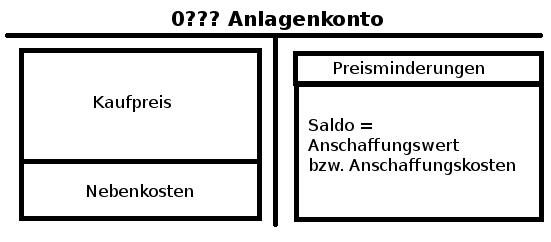
\includegraphics[width=10cm]{Bilder/Anlagenaktivierung}
\caption{Konto bei der Aktivierung der Anlage}%
\end{figure}
Wie die Grafik zeigt, ergibt der Saldo des Anlagenkontos den
Anschaffungswert.

\subsection{Herstellungskosten}
Werden Anlagen selbst erzeugt, dann werden die Herstellungskosten als
Anschaffungskosten herangezogen.


\chapter{Ermittlung der Abschreibung}
\thispagestyle{fancy}
Erklärungen für die Begriffe in diesem Kapitel
siehe~\autoref{sec:restwert} bis~\autoref{sec:buchwert}.

\section{Betriebliche Nutzungsdauer}
Die Abschreibung ist abhängig von der Nutzungsdauer. Die
betriebsgewöhnliche Nutzungsdauer ist der Zeitraum in Jahren, in der
die Anlage vorrausichtlich genutzt werden kann. In der Regel ist sie
kürzer als die technische Lebensdauer und hängt von Schätzungen und
Erfahrungen ab. Dabei sind aber die vom Finanzamt anerkannten
Nutzungszeiten zu beachten, da mit den Abschreibungen der Gewinn
reguliert werden kann.

\begin{table}[h]
  \centering
  \begin{tabular}{l r}
    Anlage & Jahre\\
    \hline
    Gebäude & 33$^1/_3$\\
    Maschinen & 5 - 10\\
    Büroausstattung & 10\\
    EDV-Anlagen und Software & 3-5\\
    Pkw und Kombis mindestens & 8\\
  \end{tabular}
  \caption{Beispiele für die Nutzungsdauer}
\end{table}

Für eine Tabelle von verschiedenen Anlagen und deren Nutzungsdauer
siehe~\autoref{sec:afatabelle} -~\nameref{sec:afatabelle}.

\section{Halbjahresregel}
\label{sec:halbjahresregel}
Für die Berechnung des Abschreibungsbetrags für das erste und letzte
Nutzungsjahr ist das Datum der \textbf{Inbetriebnahme}
maßgeblich. Wenn die Inbetriebnahme in der ersten Hälfte des
Geschäftsjahr erfolgt, dann wird für das erste Jahr die gesamte
Jahresabschreibung verbucht. Erfolgt sie in der zweiten Hälfte, wird
im ersten Jahr nur die Hälfte und im letzten Jahr nur die Hälfte der
Jahresabschreibung verbucht.

\section{Lineare Abschreibung}
Bei der linearen Abschreibung verändern sich die Abschreibungsbeträge
über die gesamte Nutzungdauer nicht. Eine Ausnahme ist der letzte
Abschreibungsbetrag: sollte die Anlage nach der Nutzungsdauer nicht
aus dem Betrieb ausgeschieden werden, dann wird der
Abschreibungsbetrag um \euro{} 1,- verringert, um den Erinnerungseuro
auf dem Anlagenkonto zu behalten. Dieser Erinnerungseuro wird erst
nach der Ausscheidung der Anlage abgeschrieben.
\par

Die lineare Anlagenabschreibung ist vom Steuerrecht zwingend
vorgeschrieben und ist somit in der Praxis die am häufigsten
auftretende Abschreibungsart.

\section{Substanzabschreibung}
Die Substanzabschreibung setzt den Wert des Grundstückes bzw. der
Förderrechte in Beziehung zur Gesamtmenge der abbäufähigen
Substanz. Letzteres muss bei der Anschaffung geschätzt werden.
\par

Relevant ist sie somit für Unternehmen, die Bodenschätze gewinnen, da
ein Gründstuck mit einer abgebauten Substanz an wert verliert. Laut
dem Steuerrecht müssen Bergbauunternehmen, Steinbrüche und andere
Betriebe, die einen Verbrauch der Substanz mit sich bringen diese Art
der Abschreibung durchführen.
\par

\begin{equation}
  \label{eq:2}
  { \text{Anschaffungswert} \over \text{abbaufähige
Substanz} } \cdot \text{Fördermenge}
\end{equation}


\chapter{Anlagenbuchführung}
Im Hauptbuch sind die Anlagen auf ihren Konten bereits erfasst.  Die
Einzelerfassung der Anlagen in der Anlagenbuchführung ist jedoch
erforderlich:
\begin{itemize}
  \item Zur Kontrolle des Anlagenbestandes.
  \item Zur Ermittlung der Abschreibung.
  \item Im Interesse der Kostenrechnung.
\end{itemize}

Das Anlagenverzeichnis muss, laut Steuergesetz, erst zum Zeitpunkt der
Abgabe an das Finanzamt ordnungsgemäß geführt sein. Dies ist natürlich
nicht sehr ratsam, da das Unternehmen aus ordentlich geführten Büchern
immer profitieren kann. Sollte es gar nicht geführt werden, verletzt
man die Aufzeichnungspflicht und kann mit einer Strafe rechnen.
\\\\
Dinge die in einem Anlagenverzeichnis vorhanden sein sollten:
\begin{multicols}{2}
  \begin{itemize}
    \item Laufende Nummer oder Inventarnummer
    \item Datum der Anschaffung (Herstellung) und der Inbetriebnahme
    \item Art der Anlage
    \item Name und Anschrift des Lieferanten
    \item Anschaffungswert
    \item voraussichtliche Nutzungsdauer
    \item Abschreibungssatz
    \item jährlicher Abschreibungsbetrag
    \item Buchwert am Ende der Rechnungsperiode
  \end{itemize}
\end{multicols}

\section{Anlagendatei}
\label{sec:anlagendatei}
Die Anlagendatei ist die Anlagenbuchführung mit Hilfe einer
Datenverarbeitungsanlage. Diese Art wird von allem von mittleren und
großen Unternehmen bevorzugt.

Vorteile:
\begin{itemize}
  \item Suchfunktionen erleichtern das Wiederfinden von Anlagen.
  \item Zusätzliche Daten können zu der Anlage erfasst werden
(z.B. Leistungswert, Garantiezeiten etc.).
  \item Die Berechnung des Abschreibungsbetrags erfolgt automatisch.
  \item Ist das System Teil eines größeren FiBu(ERP)-Systems, können
die ermittelten Werte gleich für die restliche Buchhaltung verwendet
werden
\end{itemize}

Nachteile:
\begin{itemize}
  \item Hohe Kosten für das System
\end{itemize}

\section{Anlagenverzeichnis}
\label{sec:anlagenverzeichnis}
Das Anlagenverzeichnis ist die Anlagenbuchführung die manuell
verwaltet wird. Dabei wird für jedes Jahr, in dem Anschaffungen
erfolgen, ein neues Datenblatt begonnen. In den Datenblättern werden
dann die Abschreibungsbeträge und Buchwerte berechnet. Diese Art ist
besonders von Kleinunternehmen bevorzugt, da sie kostengünstig
ist. Die Nachteile sind die Vorteile einer Anlagendatei
(siehe~\autoref{sec:anlagendatei} -~\nameref{sec:anlagendatei}).


\chapter{Verbuchung der Abschreibung}
\thispagestyle{fancy}
Abschreibungen sind verpflichtend vorzunehmen und eine versäumte
Buchung kann nicht nachgeholt werden!

\section{Direkte Abschreibung}
\label{sec:direkteabschreibung}
Am Jahresende wird der Abschreibungbetrag direkt vom Anlagenkonto
abgebucht. Dabei wird das Aufwandskonto \textit{7010 Abschreibungen
von Sachanlagen} verwendet. Dies unterstreicht noch einmal, dass die
Abschreibung Gewinn mindernd ist.

\begin{figure}[h]
  \caption{Verbuchung einer Abschreibung}
  \begin{equation*}
    \begin{array}{l}
      \text{7010 Abschreibungen von Sachanlagen}\\
    \end{array}
    \left\slash
      \begin{array}{l}
        \text{0??? Anlagenkonto}\\
      \end{array}
    \right.
  \end{equation*}
  \label{fig:abschreibungsbuchung}
\end{figure}

Aus dieser Buchung ergibt sich für die Bilanz ein solches Gebilde:
\begin{figure}[ht]
\centering
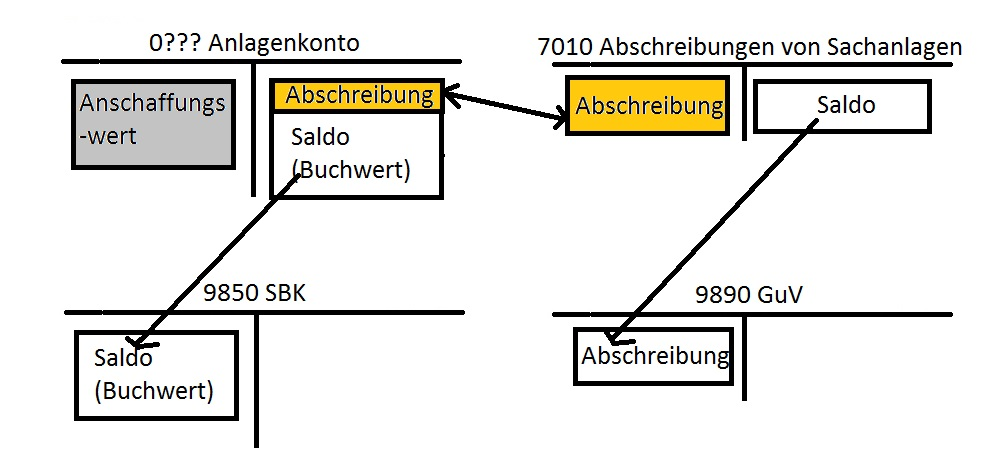
\includegraphics[width=12cm]{Bilder/Abschreibung-Konten_der_Bilanz}
\caption{Zusammenhang der Konten bei der Abschreibung}
\end{figure}
\pagebreak

Merkmale der Abschreibung:
\begin{itemize}
  \item Am Anlagenkonto scheint der Buchwert auf.
  \item Der Anschaffungswert und die vorrangegangenen Abschreibungen
sind nur aus dem Anlagenverzeichnis ersichtlich.
\end{itemize}

\section{Indirekte Abschreibung}
\label{sec:indirekteabschreibung}
Bei der Indirekten Abschreibung wird die Abschreibung nicht vom
Anlagenkonto abgebucht, sondern von einem Stellvertreter Konto in der
Klasse 0. Somit ergibt sich für jedes \textit{0??? Anlagenkonto} ein
\textit{0??? Kumulierte Abschreibungen zu 0???}. Der Buchungsatz der
eigentlichen Abschreibung lautet dann:

\begin{equation*}
  \begin{array}{l}
    \text{7010 Abschreibungen von Sachanlagen}\\
  \end{array}
  \left\slash
    \begin{array}{l}
      \text{0??? Kumulierte Abschreibungen zu 0???}\\
    \end{array}
  \right.
\end{equation*}

Da am Ende des Jahres auf dem Konto \textit{0??? Kumulierte
Abschreibungen zu 0???} ein Habensaldo entsteht, wandert es auch auf
die Passiva. Dies bewirkt den selben Effekt wie bei der direkten
Abschreibung - der Wert der Anlage wird um die Abschreibungen
verringert und somit auch die Bilanzsumme.\\
\\
Zur Illustration die Abschreibung einer Maschine:
\begin{figure}[ht]
\centering
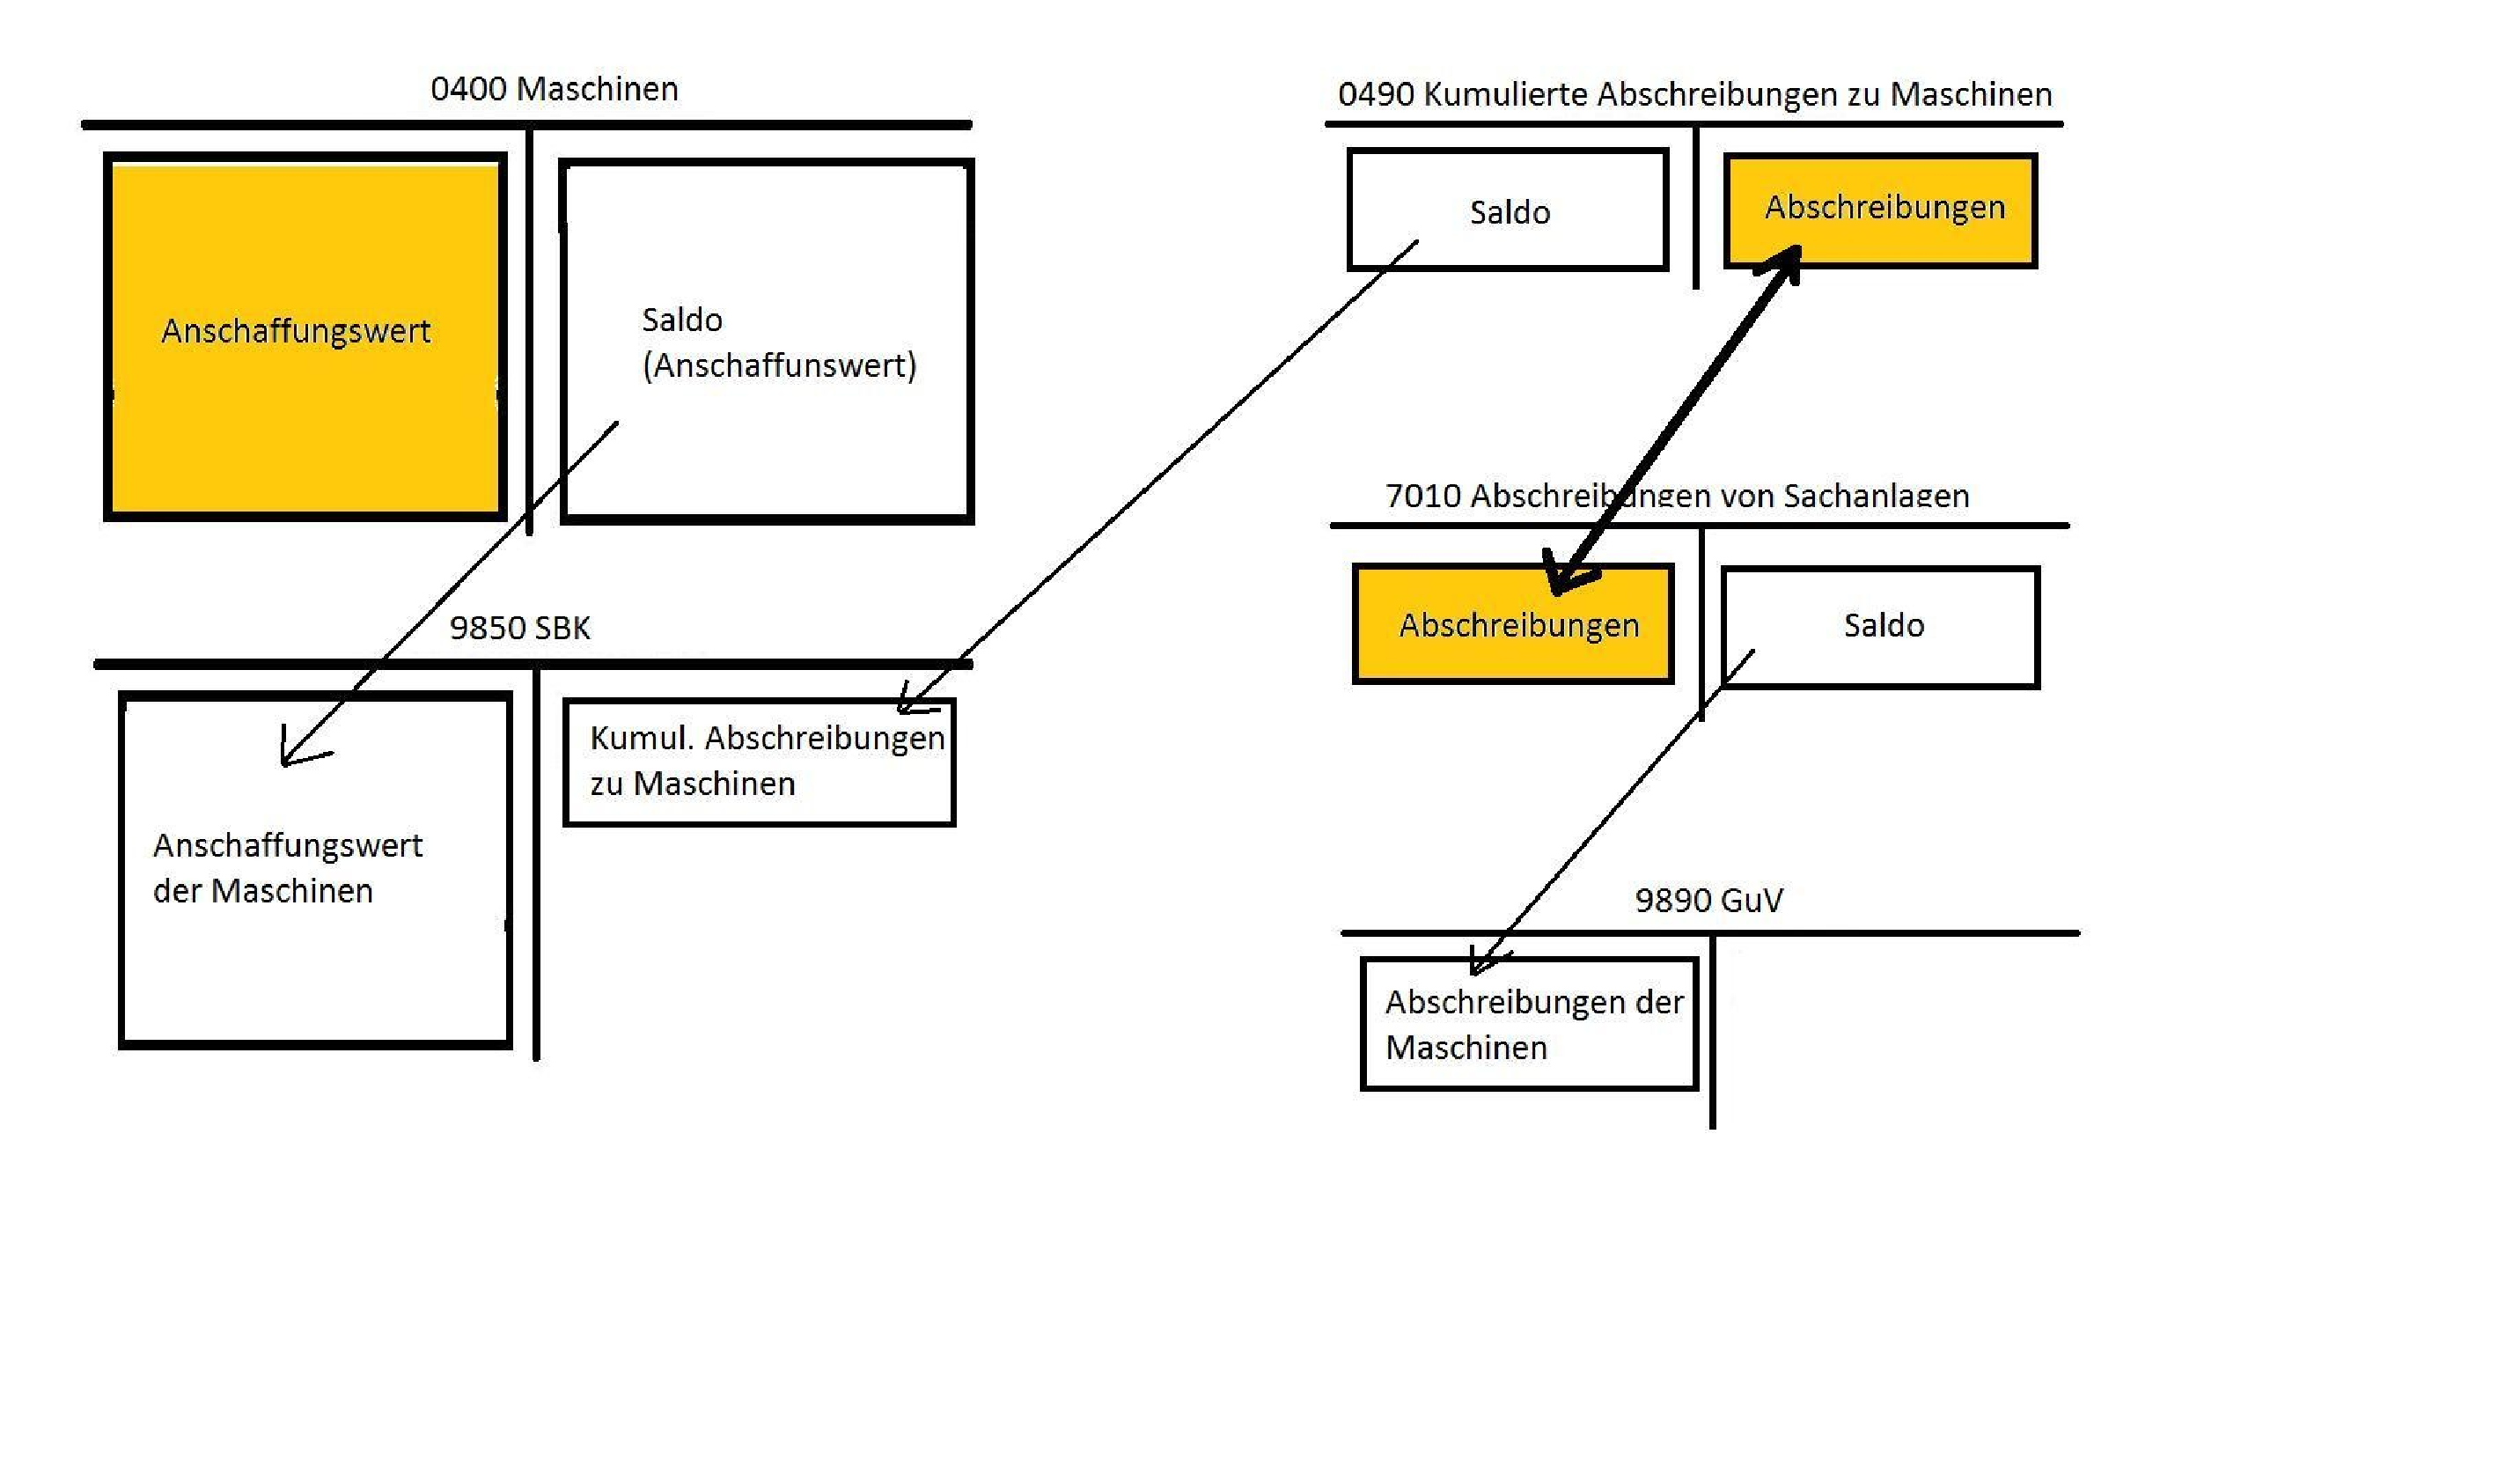
\includegraphics[width=14cm]{Bilder/IndirekteAbschreibung-Konten_der_Bilanz}
\caption{Zusammenhang der Konten der indirekten Abschreibung}
\end{figure}

\subsection{Verbuchung von Anlagenverkäufen bei indirekter Abschreibung}
Die Buchungen sind im allgemeinen gleich mit den
in~\autoref{sec:verkaufsausscheidung}
-~\nameref{sec:verkaufsausscheidung} beschriebenen Buchungen. Die
Unterschiede sind:
\begin{itemize}
  \item { Die Finale Abschreibung läuft wie
in~\autoref{sec:indirekteabschreibung}
-~\nameref{sec:indirekteabschreibung} beschrieben ab.
    }
  \item { Vor dem Ausbuchen der Anlage
(siehe~\autoref{subsec:anlagsausbuchung}
-~\nameref{subsec:anlagsausbuchung}) wird noch das Konto \textit{0???
Kumulierte Abschreibungen zu 0???}  aufgelöst. Dies erfolgt mit der
Buchung:
\begin{equation*}
  \begin{array}{l}
    \text{0??? Kumulierte Abschreibungen zu 0???}\\
  \end{array}
  \left\slash
    \begin{array}{l}
      \text{0??? Anlagenkonto}\\
    \end{array}
  \right.
\end{equation*}
}
\end{itemize}

\begin{figure}[ht]
\centering
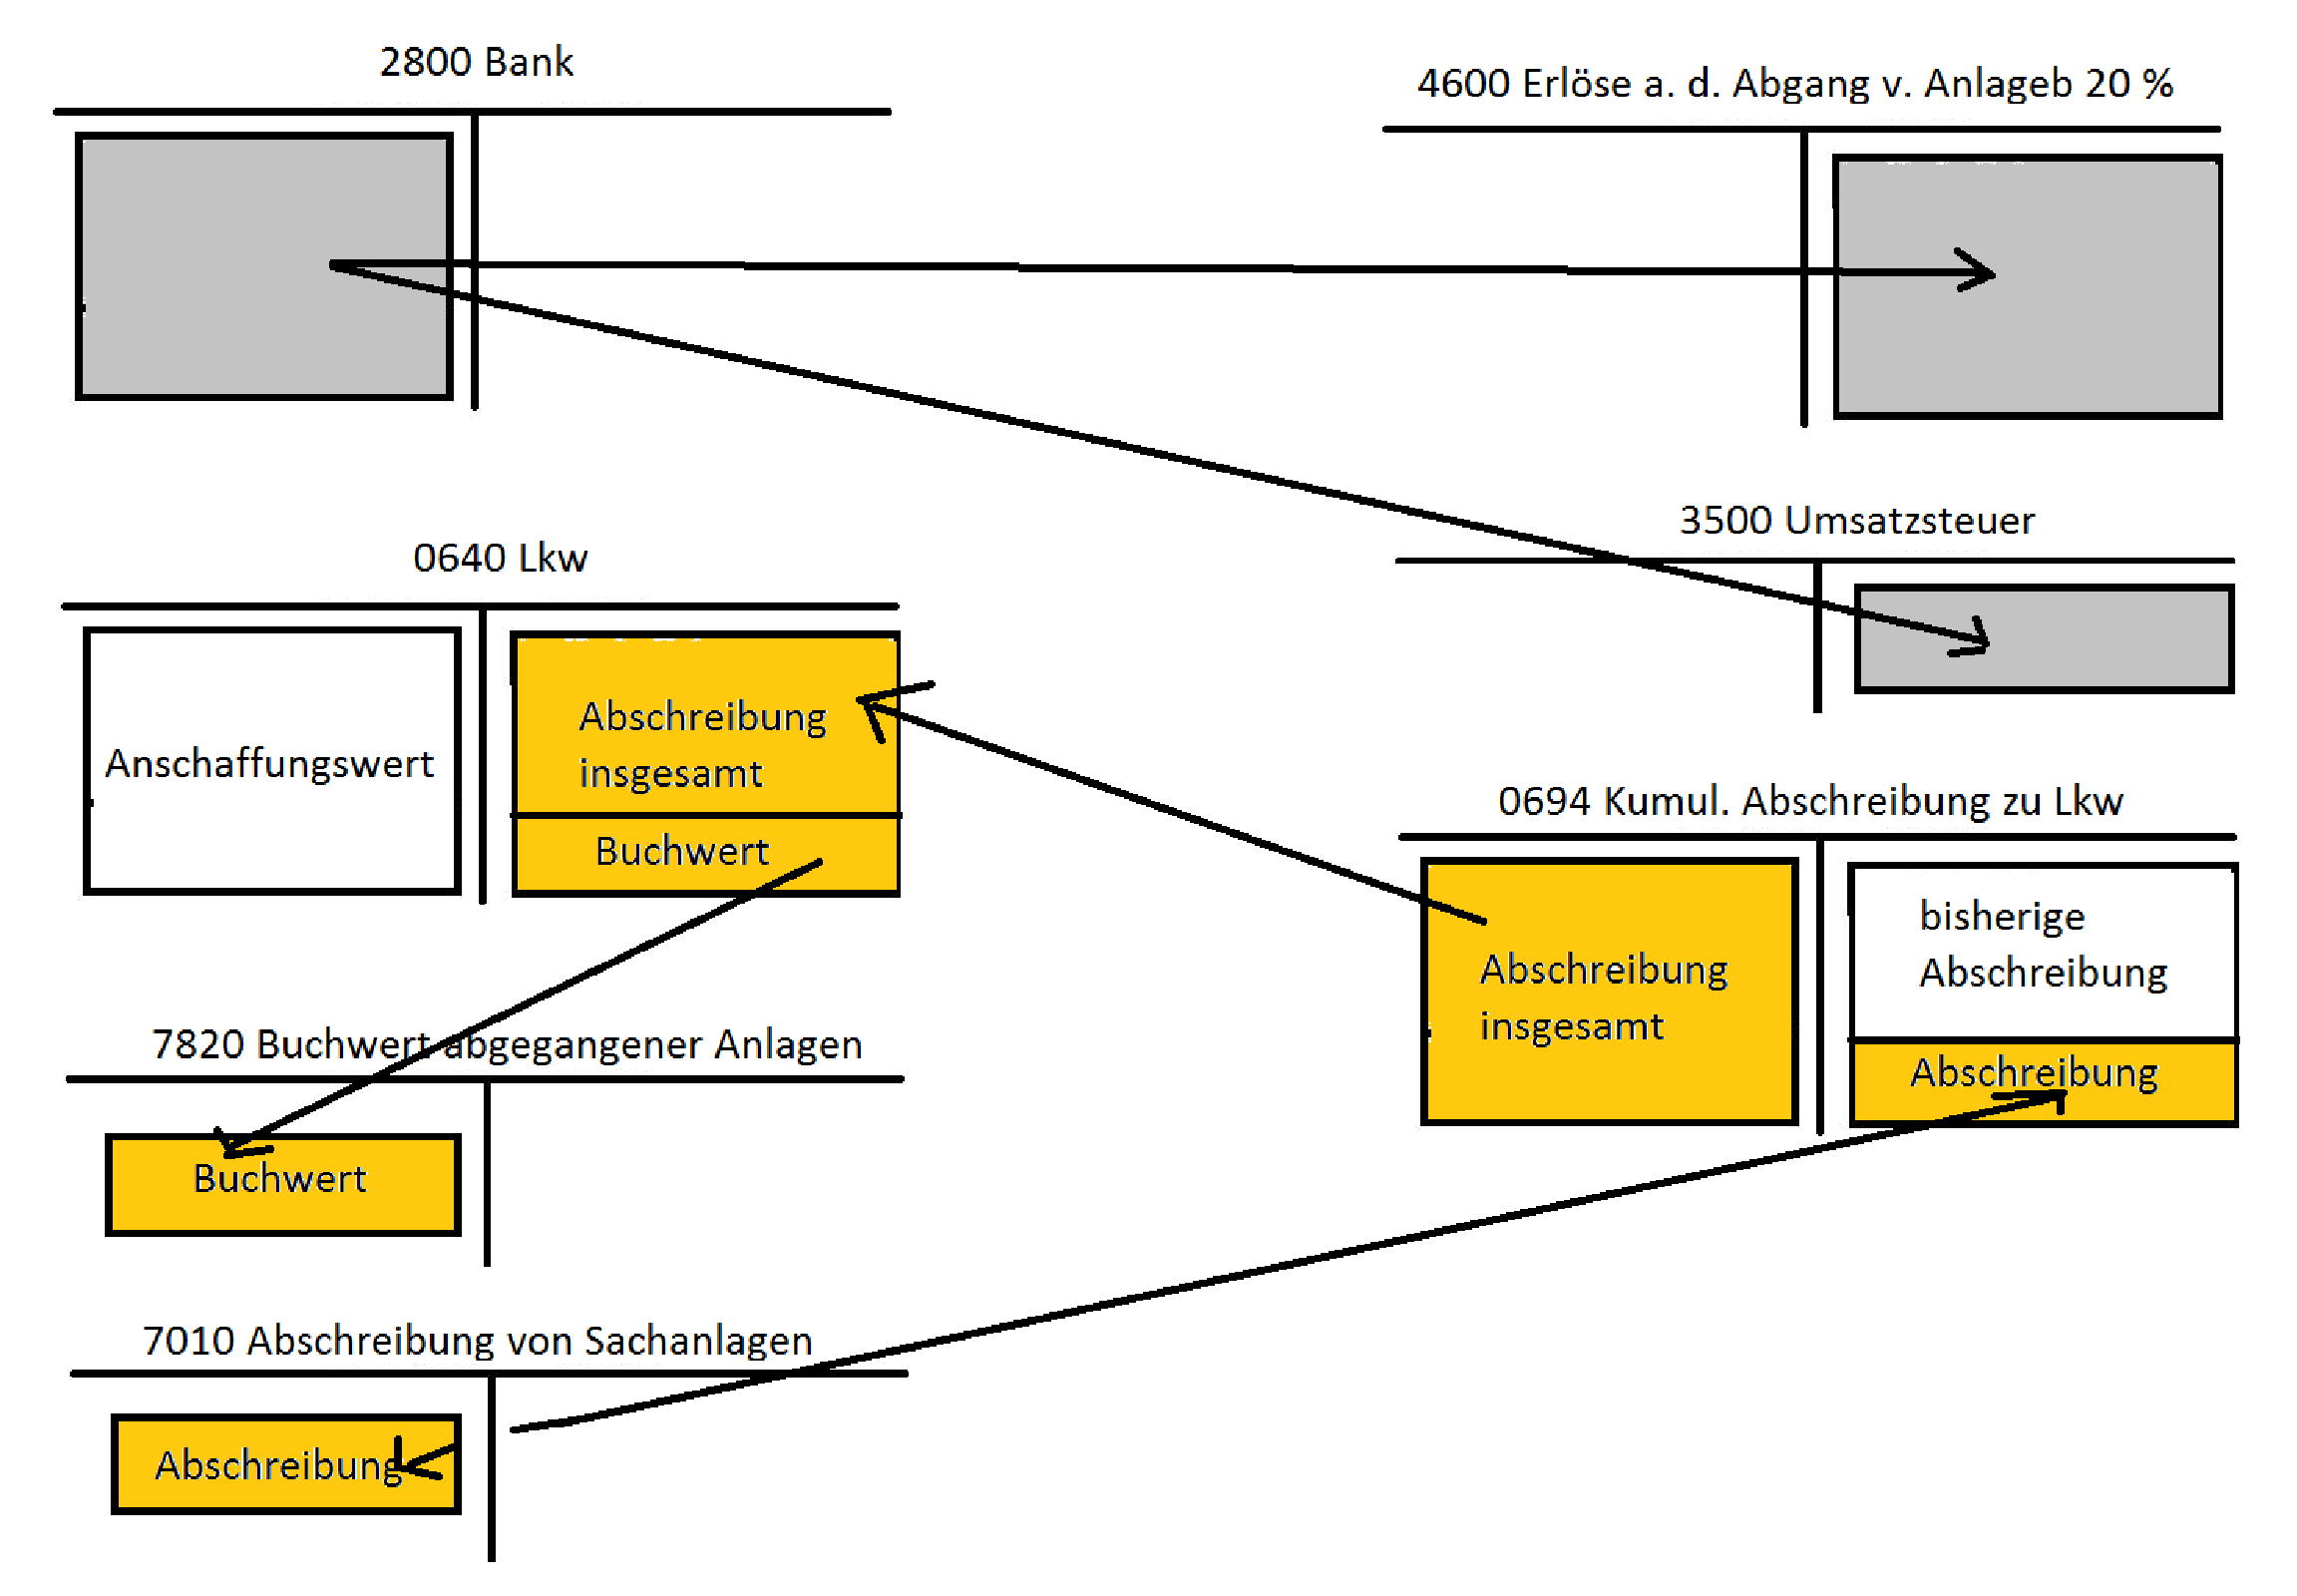
\includegraphics[width=14cm]{Bilder/IndirekteAusbuchung-Konten_der_Bilanz}
\caption{Zusammenhang der Konten bei dem Verkauf bei der indirekten Abschreibung}
\end{figure}

\section{Geringwertige Wirtschaftsgüter}
\label{sec:geringwertigewirtschaftsgueter}
Geringwertige Wirtschaftsgüter sind laut EStG abnutzbare Anlagegüter,
deren Anschaffungs-/Herstellungswert den Wert von \euro{} 400,-
(exkl. USt) nicht übersteigen. Sie können, müssen aber nicht, im Jahr
der Anschaffung voll abgeschrieben werden. Dabei ist zu beachten, dass
Wirtschaftsgüter, die aus Teilen bestehen, als Einheit aufzufassen
sind, wenn sie nach ihrem wirtschaftlichen Zweck eine Einheit
bilden. Das bedeutet, dass diese Güter nicht getrennt als
,,geringwertig'' verbucht werden können.
\par
Sollte ein geringwertiges Wirtschaftsgut nicht voll abgeschrieben
werden, so ist die Abschreibung normal durchzuführen (in Beziehung zur
Nutzungsdauer).\\
\\
Es gibt zwei Arten die geringwertigen Anlagen zu verbuchen:
\begin{itemize}
  \item { \textbf{Abschreibung zum Jahresende} }
  \begin{itemize}
    \item { Sofortige Buchung beim Kauf:\\
        \begin{equation*}
          \begin{array}{l}
            \text{0??? Geringwertige ...}\\
            \text{2500 Vorsteuer}\\
          \end{array}
          \left\slash
            \begin{array}{l}
              \text{33??? Lieferantenkonto (oder 2800 Bank etc.)}\\
            \end{array}
          \right.
        \end{equation*}
      }
    \item { Buchung am Jahresende:\\
        \begin{equation*}
          \begin{array}{l}
            \text{7030 Abschreibung geringwertiger Wirtschaftsgüter}\\
          \end{array}
          \left\slash
            \begin{array}{l}
              \text{0??? Geringwertige ...}\\
            \end{array}
          \right.
        \end{equation*}
      }
  \end{itemize}
  \item { \textbf{Sofortige Abschreibung beim Kauf}\\
      \begin{equation*}
        \begin{array}{l}
          \text{7030 Abschreibung geringwertiger Wirtschaftsgüter}\\
          \text{2500 Vorsteuer}\\
        \end{array}
        \left\slash
          \begin{array}{l}
            \text{33??? Lieferantenkonto (oder 2800 Bank etc.)}\\
          \end{array}
        \right.
      \end{equation*}
  }
\end{itemize}

\chapter{Andere Buchungen}
\thispagestyle{fancy}
\section{Selbst erstellte Anlagen}
Alle anfallenden Kosten für die Herstellung einer Anlage werden normal
auf die dazu gehörigen Aufwandskonten verbucht
(z.B. Rohstoffverbrauch, Personalaufwand). Nach der Fertigstellung der
Anlage werden die Herstellungskosten als Ertrag, mit dem Konto 4850
Aktivierte Eigenleistungen, auf das Anlagenkonto verbucht. Somit
werden die Aufwendungen neutralisiert.\\
\\
Der Buchungsatz zur Erfassung der selbst erstellten Anlage:
\begin{equation*}
  \begin{array}{l}
    \text{0??? Anlagenkonto}\\
  \end{array}
  \left\slash
    \begin{array}{l}
      \text{4850 Aktivierte Eigenleistungen}\\
    \end{array}
  \right.
\end{equation*}

\begin{figure}[ht]
\centering
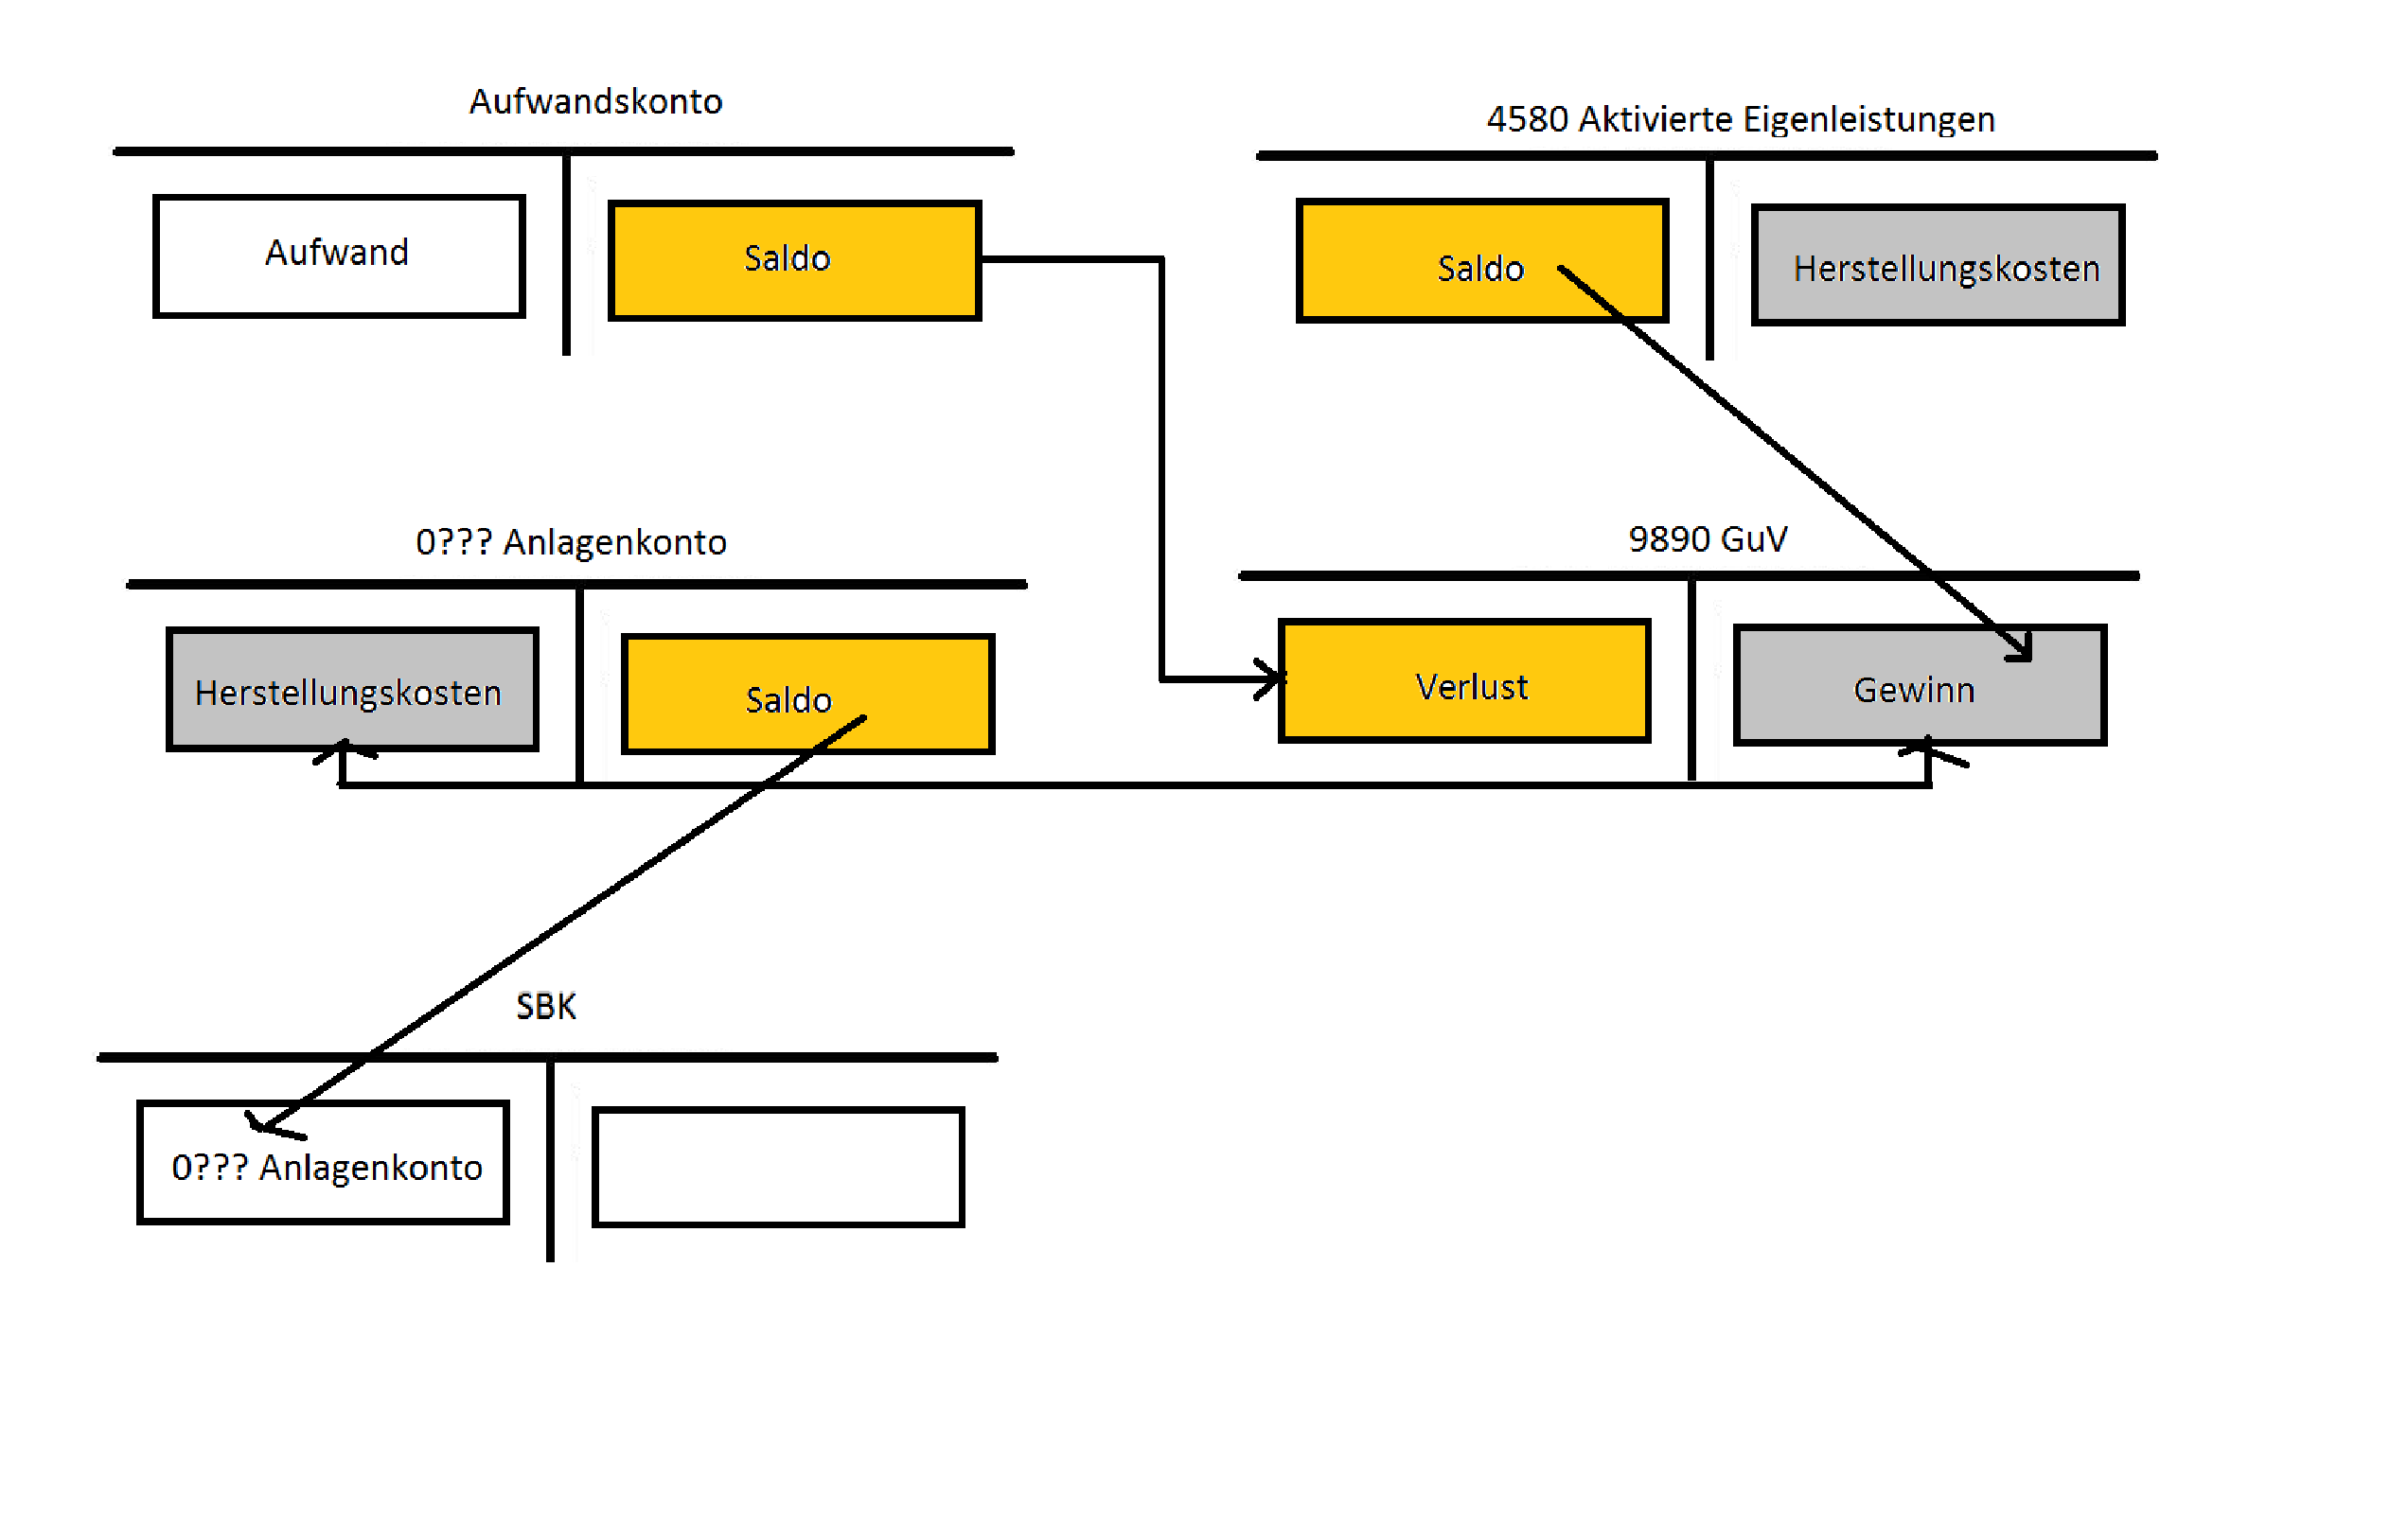
\includegraphics[width=14cm]{Bilder/Eigenleistung-Konten_der_Bilanz}
\caption{Zusammenhang der Konten bei der Verbuchung einer selbst
erstellten Anlage}
\end{figure}

\section{In Bau befindliche Anlagen}
Anlagen, die zum Abschlussstichtag, noch nicht fertiggestellt sind,
sind definiert als ,,Anlagen im Bau''. Aufwendungen für die unfertigen
Anlagen werden auf dem eigenen Konto 0710 Anlagen im Bau
ausgewiesen. Die planmäßige Abschreibung darf aber auch hier erst mit
dem Zeitpunkt der Inbetriebnahme beginnen.\\

\subsection{Buchungen während der Herstellung}
Buchung einer Teilzahlung:
\begin{equation*}
  \begin{array}{l}
    \text{0710 Anlagen im Bau}\\
    \text{2500 Vorsteuer}\\
  \end{array}
  \left\slash
    \begin{array}{l}
      \text{4850 Aktivierte Eigenleistungen}\\
    \end{array}
  \right.
\end{equation*}
\\
Buchung bei selbst erstellten Teilen:
\begin{equation*}
  \begin{array}{l}
    \text{0710 Anlagen im Bau}\\
  \end{array}
  \left\slash
    \begin{array}{l}
      \text{33??? Lieferantenkonto (oder 2800 Bank etc.)}\\
    \end{array}
  \right.
\end{equation*}

\subsection{Buchungen nach der Fertigstellung}
Es erfolgt eine Umbuchung auf das entsprechende Anlagenkonto, um die
gesamten Kosten der Anlage zu erfassen:
\begin{equation*}
  \begin{array}{l}
    \text{0??? Anlagenkonto}\\
  \end{array}
  \left\slash
    \begin{array}{l}
      \text{0710 Anlagen im Bau}\\
    \end{array}
  \right.
\end{equation*}

\chapter{Instandhaltung von Anlagen}
\thispagestyle{fancy}
Anlagen müssen meist nach einer bestimmten Zeit gewartet werden um die
Bertiebsfähigkeit zu erhalten. Dabei ist wichtig zu erwähnen, dass der
Wert der Anlage nicht ersichtlich gesteigert wird, da es sich nur um
eine Wartung bzw. Servicearbeiten handelt, auch wenn z.B. ein Teil der
Anlage durch ein höherwertiges Material ersetzt wird. Im Zweifelsfall
gilt es als Instandhaltung, wenn:
\begin{itemize}
  \item der ordnungsgemäße Zustand erhalten wird
  \item die Wesensart der Anlage nicht verändert wird
\end{itemize}

Die Aufwendungen für eine Instandhaltung sind noch im Jahr der
Aufwendung voll ,,abschreibbar''. Hierfür wird aber nicht das Konto
\textit{7010 Abschreibungen von Sachanlagen}, sondern \textit{7200
Instandhaltung} durch Dritte, verwendet. Da keine Wertsteigerung der
Anlage vorherrscht, sieht der Buchungsatz mit dem Beleg des
Wartungsdienstes etc. dann gefolgt aus:
\begin{equation*}
  \begin{array}{l}
    \text{7200 Instandhaltung durch
Dritte}\\
     \text{2500 Vorsteuer}\\
  \end{array}
  \left\slash
    \begin{array}{l}
      \text{33??? Lieferantenkonto (oder 2800 Bank etc.)}\\
    \end{array}
  \right.
\end{equation*}

\chapter{Erweiterung einer Anlage}
\thispagestyle{fancy}
Wenn eine sichtliche Erweiterung einer Anlage stattfindet, dann muss
dieser Herstellungsaufwand auf das entsprechende Konto der Klasse 0
verbucht werden. Der aktivierungspflichtige Betrag (=
Herstellungsaufwand) wird dann wie eine Anschaffung verbucht
(siehe~\autoref{eq:anschaffungsbuchung}~\nameref{eq:anschaffungsbuchung}). Mit
der Änderung des Anlagenwertes verändert sich auch die
Restnutzungsdauer des Anlagegutes und auch entsprechend auch der
Abschreibungsbetrag. Der Abschreibungsbetrag wird aus dem neuen
Anlagenwert und der Restnutzungsdauer berechnet:
\begin{equation}
  { {Anschaffungskosten + Erweiterungskosten } \over Restnutzungsdauer
  } = neuer Abschreibungsbetrag
  \end{equation}
\\\\
Eine Aktivierungspflicht liegt vor, wenn:
\begin{itemize}
  \item die Anlage durch eine Aufwendung in seiner Substanz vermehrt wird
  \item die Gebrauchsmöglichkeit einer Anlage wird wesentlich verändert
\end{itemize}

\chapter{Ausscheiden einer Anlage}
\thispagestyle{fancy}
\section{Ausscheidung bei einem Verkauf}
\label{sec:verkaufsausscheidung}
Bei einem Verkauf, erhält der Verkäufer Geld und der Käufer im
Gegenzug eine Anlage. Da es sich bei dem so gewonnenen Geld um einen
Erlös handelt, wird nicht einfach \textit{20??? Forderungskonto (oder
2800 Bank etc.) / 0??? Anlagenkonto} gebucht! Der Verkauf wird, im
Prinzip, wie ein Handelswarenverkauf verbucht. Hierfür werden das
Konto \textit{4600 Erlöse aus dem Abgang von Anlagen 20 \%} bzw. bei
Pkw, Kobmis und Krafträdern \textit{4601 Erlöse aus dem Abgang von
Anlagen 0 \%} benötigt.

\begin{figure}[h]
  \centering
  \begin{equation*}
    \begin{array}{l}
      \text{20??? Forderungskonto (oder 2800 Bank etc.)}\\
    \end{array}
    \left\slash
      \begin{array}{l}
        \text{4600 Erlöse aus dem Abgang von Anlagen}\\
        \text{3500 Umsatzsteuer}\\
      \end{array}
    \right.
  \end{equation*}
  \caption{Verbuchung eines Anlagenverkaufs}
\end{figure}

\subsection{Ausbuchung der Anlage}
\label{subsec:anlagsausbuchung)}
Da sich die Anlage noch auf dem Anlagenkonto befindet, muss dieser
ausgebucht werden. Vorher müssen aber noch eine etwaige Abschreibung
verbucht werden. Hierbei gilt wieder die Halbjahresregel
(siehe~\autoref{sec:halbjahresregel} -~\nameref{sec:halbjahresregel})!
Nach der Abschreibung wird der Buchwert auf das Konto \textit{7820
Buchwert abgegangener Anlagen} verbucht.\\
\\
Für die die Abschreibung zum Zeitpunkt des Verkaufs
siehe~\autoref{fig:abschreibungsbuchung}
-~\nameref{fig:abschreibungsbuchung}.

\begin{figure}[h]
  \centering
  \begin{equation*}
    \begin{array}{l}
      \text{7820 Buchwert abgegangener Anlagen}\\
    \end{array}
    \left\slash
      \begin{array}{l}
        \text{0??? Anlagenkonto}\\
      \end{array}
    \right.
  \end{equation*}
  \caption{Ausbuchen des Buchwerts}
  \label{fig:buchwertsausbuchung}
\end{figure}

\subsection{Durchführung der Saldierungsbuchung}
\label{sec:verkaufssaldierung}
Die Saldierung der Verkaufserklöse und der Buchwerte aus
Anlagenverkäufe is nur bei Kapitalgesellschaften vorgeschrieben. Dabei
wird zwischen den Konten \textit{4600 Erlöse aus dem Abgang von
Anlagen} und \textit{7820 Buchwert abgegangener Anlagen} und dem Konto
\textit{9890 GuV} ein weiteres Konto geschaltet, welches entweder den
Gewinn oder den Verlust darstellt. Welche Buchungen erfolgen, gibt der
Saldo der Verkaufserlöse und der Buchwerte an:
\begin{table}[h]
  \centering
  \begin{tabular}{l r}
    & Verkaufserlöse\\
    - & Buchwerte\\
    \hline
    & Saldo
  \end{tabular}
\end{table}

\subsubsection{Gewinnbuchung bei positiven Saldo}
Wenn der ermittelte Saldo positiv oder Null ist, dann erfolgen
folgende Buchungen:\\
\\
Umbuchung des Verkaufserlöses:
\begin{equation*}
  \begin{array}{l}
    \text{4600 Erlöse aus dem Abgang von Anlagen}\\
  \end{array}
  \left\slash
    \begin{array}{l}
      \text{4630 Erträge aus dem Abgang von Anlagen}\\
    \end{array}
  \right.
\end{equation*}\\
\\
Umbuchung des Buchwertes:
\begin{equation*}
  \begin{array}{l}
    \text{4630 Erträge aus dem Abgang von Anlagen}\\
  \end{array}
  \left\slash
    \begin{array}{l}
      \text{7820 Buchwert abgegangener Anlagen}\\
    \end{array}
  \right.
\end{equation*}

\begin{figure}[ht]
\centering
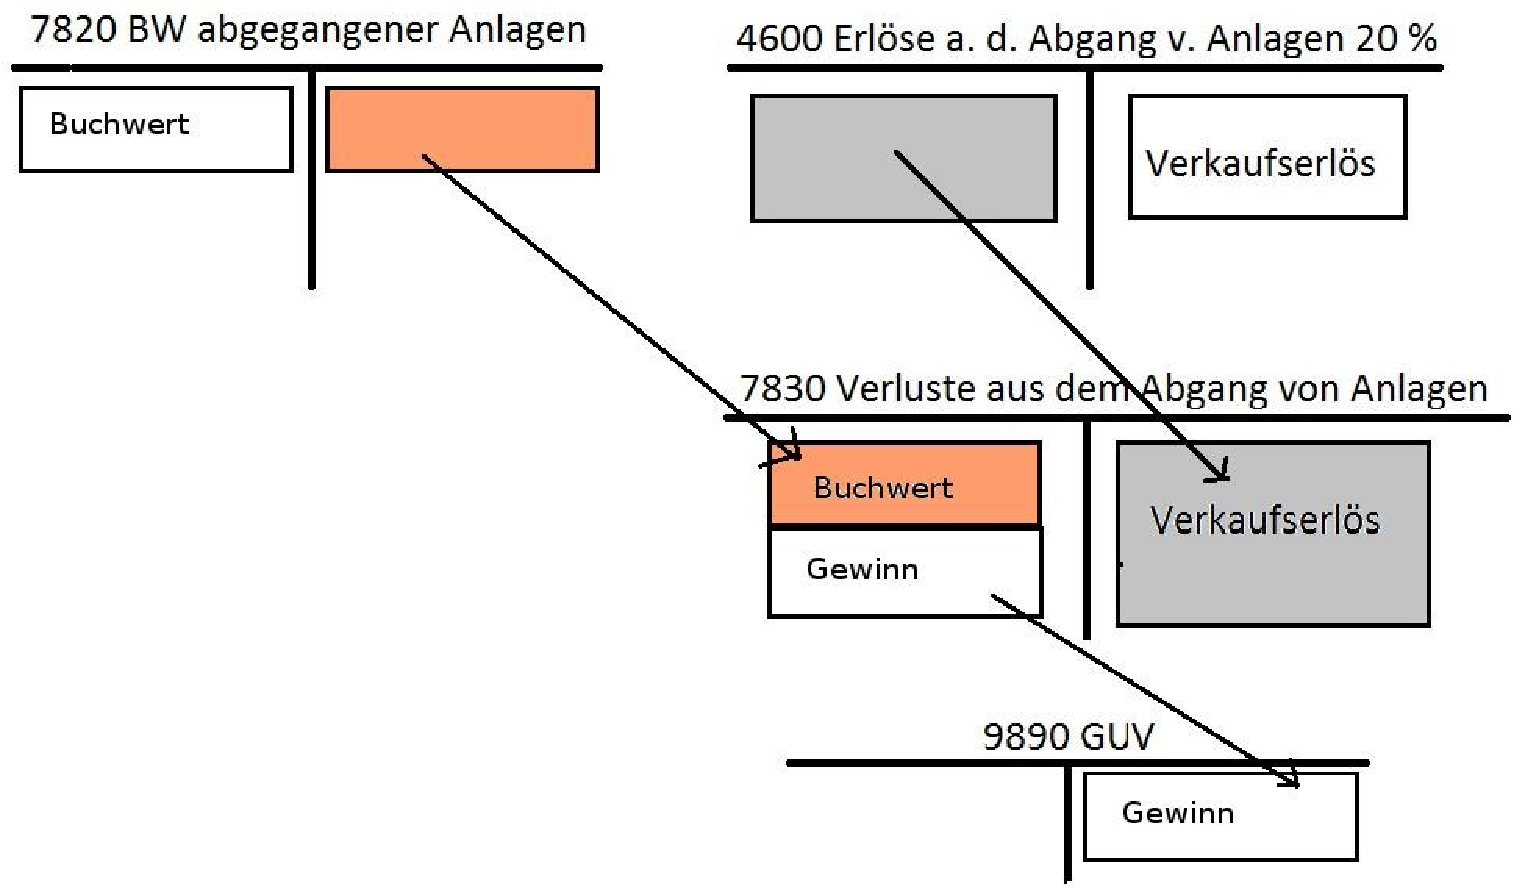
\includegraphics[width=14cm]{Bilder/Gewinnumbuchung-Konten_der_Bilanz}
\caption{Zusammenhang der Konten bei der Verbuchung eines positiven
Saldos}
\end{figure}
\pagebreak

\subsubsection{Verlustbuchung bei negativen Saldo}
Umbuchung des Verkaufserlöses:
\begin{equation*}
  \begin{array}{l}
    \text{4600 Erlöse aus dem Abgang von Anlagen}\\
  \end{array}
  \left\slash
    \begin{array}{l}
      \text{7830 Verluste aus dem Abgang von Anlagen}\\
    \end{array}
  \right.
\end{equation*}\\
\\
Umbuchung des Buchwertes:
\begin{equation*}
  \begin{array}{l}
    \text{7830 Verluste aus dem Abgang von Anlagen}\\
  \end{array}
  \left\slash
    \begin{array}{l}
      \text{7820 Buchwert abgegangener Anlagen}\\
    \end{array}
  \right.
\end{equation*}

\begin{figure}[ht]
\centering
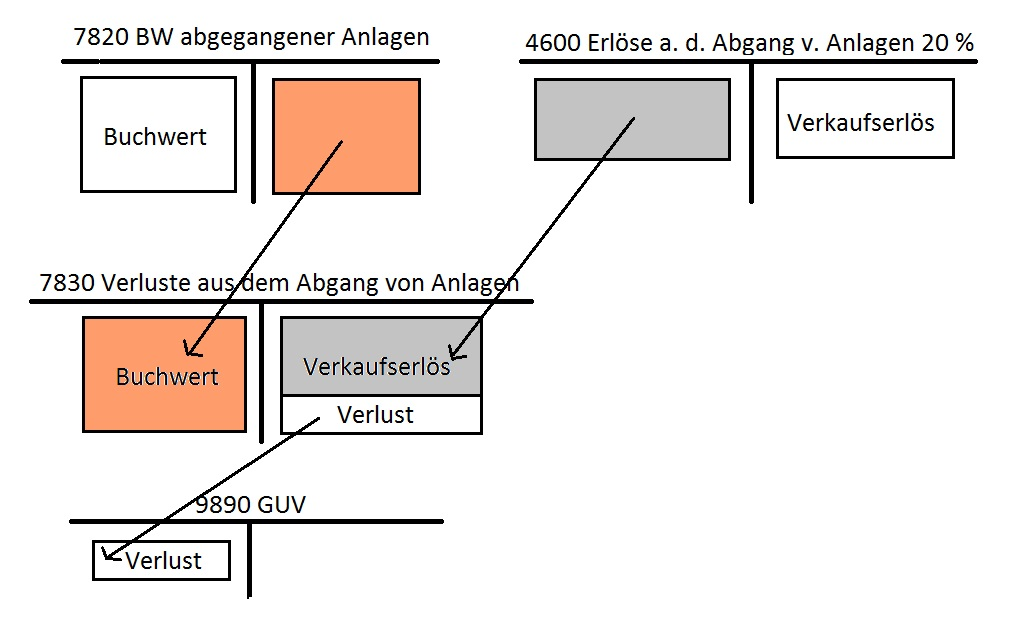
\includegraphics[width=14cm]{Bilder/Verlustsumbuchung-Konten_der_Bilanz}
\caption{Zusammenhang der Konten bei der Verbuchung eines negativen
Saldos}
\end{figure}
\pagebreak

\section{Ausscheidung bei einem Schadensfall}
\subsection{Verbuchung einer Versicherungsentschädigung}
Sollte eine Anlage, die kaputt gegangen ist, versichert gewesen sein,
so ist der erhaltene Betrag als Erlös zu verbuchen.

\begin{equation*}
  \begin{array}{l}
    \text{2800 Bank (2700 Kassa etc.)}\\
  \end{array}
  \left\slash
    \begin{array}{l}
      \text{4610 Versicherungsentschädigungen für Anlagenabgänge}\\
    \end{array}
  \right.
\end{equation*}

\subsection{Ausbuchung der Anlage}
Wie in~\autoref{sec:verkaufsausscheidung}
-~\nameref{sec:verkaufsausscheidung}, erfolgt auch beim Schadensfall
eine Ausbuchung der Anlage. Der Unterschied liegt lediglich darin,
dass der Buchwert auf das Konto \textit{7819 Sonstige Schadensfälle}
umgebucht wird, damit ersichtlich ist, dass eine Anlage durch einen
Schadensfall ausgeschieden wurde.\\
\\
Für die die Abschreibung zum Zeitpunkt des Verkaufs
siehe~\autoref{fig:abschreibungsbuchung}
-~\nameref{fig:abschreibungsbuchung}.\\
\\
Ausbuchung des Buchwertes:
\begin{equation*}
  \begin{array}{l}
    \text{7819 Sonstige Schadensfälle}\\
  \end{array}
  \left\slash
    \begin{array}{l}
      \text{0??? Anlagenkonto}\\
    \end{array}
  \right.
\end{equation*}

\subsection{}

\subsection{Durchführung der Saldierungsbuchung}
Diese ist auch hier nur für Kapitalgesellschaften eine
Pflicht.\\
\\Berechnung des Saldos:
\begin{table}[h]
  \centering
  \begin{tabular}{l r}
    & Versicherungsentschädigungen\\
    - & Schäden (Buchwerte)\\
    \hline
    & Saldo
  \end{tabular}
\end{table}

\subsubsection{Gewinnbuchung bei positiven Saldo}
Die Buchungen sind im wesentlichen gleich wie
bei~\autoref{sec:verkaufssaldierung}
-~\nameref{sec:verkaufssaldierung}, es werden nur die hierzu eigenen
Konten benutzt.\\
\\
Umbuchung der Versicherungsentschädigung
\begin{equation*}
  \begin{array}{l}
    \text{4610 Versicherungsentschädigungen für Anlagenabgänge}\\
  \end{array}
  \left\slash
    \begin{array}{l}
      \text{4630 Erträge aus dem Abgang von Anlagen}\\
    \end{array}
  \right.
\end{equation*}\\
\\
Umbuchung des Schadens (Buchwertes)
\begin{equation*}
  \begin{array}{l}
    \text{4630 Erträge aus dem Abgang von Anlagen}\\
  \end{array}
  \left\slash
    \begin{array}{l}
      \text{7819 Sonstige Schadensfälle}\\
    \end{array}
  \right.
\end{equation*}

\subsubsection{Verlustbuchung bei negativen Saldo}
Auch diese Buchungen sind im wesentlichen gleich wie
bei~\autoref{sec:verkaufssaldierung}
-~\nameref{sec:verkaufssaldierung}.\\
\\
Umbuchung der Versicherungsentschädigung
\begin{equation*}
  \begin{array}{l}
    \text{4610 Versicherungsentschädigungen für Anlagenabgänge}\\
  \end{array}
  \left\slash
    \begin{array}{l}
      \text{7830 Verluste aus dem Abgang von Anlagen}\\
    \end{array}
  \right.
\end{equation*}
\\
Umbuchung des Schadens (Buchwertes):
\begin{equation*}
  \begin{array}{l}
    \text{7830 Verluste aus dem Abgang von Anlagen}\\
  \end{array}
  \left\slash
    \begin{array}{l}
      \text{7819 Sonstige Schadensfälle}\\
    \end{array}
  \right.
\end{equation*}

\section{Ausscheidung nach voller Abschreibung}
Scheidet eine vollabgeschriebene Anlage aus dem Unternehmen aus,
erfolgt lediglich die Abschreibung des Erinnerungseuros.

\begin{equation*}
  \begin{array}{l}
    \text{7010 Abschreibungen von Sachanlagen}\\
  \end{array}
  \left\slash
    \begin{array}{l}
      \text{0??? Anlagenkonto 1,00}\\
    \end{array}
  \right.
\end{equation*}


\chapter{Glossar}
\label{chap:glossar}
\thispagestyle{fancy}
\section{Restwert bzw. Schrottwert}
\label{sec:restwert}
Dies ist der Wert der Anlage am Ende der Nutzungsdauer. Es wird bei
der letzten Buchung entweder auf Null oder \euro{} 1,-. Letzteres wird
als Erinnerungseuro bezeichnet und erst dann zu Null gebucht, wenn die
Anlage physisch aus dem Unternehmen ausscheidet.

\section{Abschreibungsbasis}
Die Abschreibungsbasis ist der Betrag, von dem abgeschrieben
wird. Normalerweise ist dies der Anschaffungswert bzw. der
Herstellungswert.

\section{Abschreibungsatz}
Dies ist die Höhe der Abschreibung in Prozent. Sie ist von der
Nutzungsdauer abhängig.
\begin{equation}
  Abschreibungsatz = { 100 \over Nutzungsdauer}
\end{equation}

\section{Abschreibungsbetrag}
Der Abschreibungsbetrag ist der Betrag, der in einem Geschäftsjahr für
eine Anlage abgeschrieben und als Aufwand verbucht wird.
\begin{equation}
  Abschreibungsbetrag = Anschaffungswert \cdot Abschreibungssatz = {
Anschaffungswert \over Nutzungsdauer }
\end{equation}

\section{Buchwert bzw. Restbuchwert}
\label{sec:buchwert}
Dies ist die Differenz zwischen Anschaffungs- bzw. Herstellungswert
und der Summe der bereits vorgenommenen Abschreibungsbeträge. Zum
Verständnis:
\begin{equation}
  Anschaffungswert (bzw. Buchwert am 1.1.) - Abschreibungsbetrag =
Buchwert am 31.12.
\end{equation}

\section{Geringwertige Wirtschtaftsgüter}
Siehe~\autoref{sec:geringwertigewirtschaftsgueter}
-~\nameref{sec:geringwertigewirtschaftsgueter}.

\section{Anlagenverzeichnis}
Siehe~\autoref{sec:anlagenverzeichnis}
-~\nameref{sec:anlagenverzeichnis}.

\section{Anlagendatei}
Siehe~\autoref{sec:anlagendatei} -~\nameref{sec:anlagendatei}.

\section{Restnutzungsdauer}
Die Restnutzungsdauer ist die Anzahl von Jahren, in der eine Anlage
noch wirtschaftlich genutzt wird.
\begin{table}[h]
  \centering
  \begin{tabular}{l r}
    & Gesamte Nutzungsdauer\\
    - & Bisherige Nutzungsdauer\\
    \hline
    & Restnutzungsdauer
  \end{tabular}
  \caption{Berechnung der Restnutzungsdauer}
\end{table}

\chapter{Anhang}
\thispagestyle{fancy}

\section{Beispiel für eine AfA-Tabelle}
\label{sec:afatabelle}
Hierbei handelt es sich um eine AfA-Tabelle des Bundesministeriums für
Finanzen der BRD. Diese Tabelle ist jedoch auch in Österreich gültig.\\
\url{http://www.bundesfinanzministerium.de/Content/DE/Standardartikel/Themen/Steuern/Weitere_Steuerthemen/Betriebspruefung/AfA-Tabellen/2000-12-15-afa-103.pdf?__blob=publicationFile&v=1}

\section{Quellen}
\begin{itemize}
  \item MANZ - Rechnungswesen \& Controlling HAK II
  \item { MANZ - Ergänzungskapitel zu RW HLT IV\\ \url{http://www.google.at/url?sa=t&rct=j&q=&esrc=s&source=web&cd=1&cad=rja&uact=8&ved=0CCEQFjAA&url=http%3A%2F%2Fwww.wissenistmanz.at%2Fsbplus%2F141216_rw_hltiv%2Fergaenzungskap_rw_hltiv.pdf%2Fdownload&ei=Ncw2VLOKFcTiywOpnIDQDQ&usg=AFQjCNEe0KEAz4V37nveOiOR-t-yeOY_0A&sig2=L8-hqnxIaIvI4exPp0U9TA&bvm=bv.76943099,d.bGQ}
}
\end{itemize}

\end{document}
